\documentclass[10pt,twocolumn,letterpaper]{article}

\usepackage{cvpr}
%\usepackage{times}
%\usepackage{algorithm}
%%\usepackage{algorithmic}
%\usepackage{algpseudocode}
%\usepackage{epsfig}
%\usepackage{graphicx}
%\usepackage{amsmath}
%\usepackage{amssymb}
%\usepackage{subfigure}

\usepackage{times}
\usepackage{xcolor}
\usepackage{soul}
\usepackage[utf8]{inputenc}
\usepackage[small]{caption}
\usepackage{amsmath}
\usepackage{float}
\usepackage{graphicx}
\usepackage{multirow}
\usepackage{algorithm}
\usepackage{algorithmic}
\usepackage{amsmath}
\usepackage{url}
\usepackage{caption}
\usepackage{subfigure}
%\usepackage{subfig}
%\usepackage{subcaption}


\usepackage[pagebackref=true,breaklinks=true,letterpaper=true,colorlinks,bookmarks=false]{hyperref}
\def\cvprPaperID{****} % *** Enter the CVPR Paper ID here
\def\httilde{\mbox{\tt\raisebox{-.5ex}{\symbol{126}}}}
\ifcvprfinal\pagestyle{empty}\fi
\begin{document}

%%%%%%%%% TITLE
\title{DRAGN: Deep Recusively AggreGation Network}

\author{First Author\\
Institution1\\
Institution1 address\\
{\tt\small firstauthor@i1.org}
\and
Second Author\\
Institution2\\
First line of institution2 address\\
{\tt\small secondauthor@i2.org}
}

\maketitle

%%%%%%%%%%%%%%%%%%%%%%%%%%% ABSTRACT %%%%%%%%%%%%%%%%%%%%%%%%%%%%%%%%%%%%
\begin{abstract}
A lot of computer vision tasks exhibit multi-instance property, in which the learning is performed at the bag-level instead of instance-level and each bag contains of multiple instances, i.e. images. Compared to traditional multi-instance learning algorithms and recent 3D deep neural networks, feature aggregation methods have the following advantages: i)more flexible, as it can be achieved in both traditional and deep learning frameworks, and ii)more versatile, as it can deal with various types of bags without temporal or spatial dependency between images.

In this study, we proposed a deep learning-based feature aggregation model, called DRAGN(Deep Recursively AggreGation Network). It consists of two components, feature aggregation unit and feature aggregation module. The feature aggregation module uses feature aggregation unit to perform iterative and stacked convolution aggregation of multiple instances, and finally output an aggregated feature.

We assess the model performance on two biomedical image processing tasks. One is the protein subcellular localization using immunofluorescence images for human cells, and the other is gene annotation using spatial gene expression images. In both the two tasks, DRAGN outperforms the existing feature aggregation methods and the state-of-the-art models for addressing these two tasks.

\end{abstract}

%%%%%%%%%%%%%%%%%%%%%%%%%%%%%%%%%% 1,introduction %%%%%%%%%%%%%%%%%%%%%%%%%%%%%%%%%%%%
\section{Introduction}

In traditional computer vision tasks, like image classification \cite{ref1, ref2, ref3}, object detection \cite{ref4, ref5}, and semantic segmentation \cite{ref6, ref7}, the inputs of computational learning models are single images. As image processing techniques develop rapidly and the storage capacity for multi-media data grows dramatically, there is an increasing need for handling higher dimensional data, such as videos and series of images. Especially, in many image processing applications, the input consists of multiple images, which determine the output jointly. For example, when we recognize person identity based on videos, each video input can be regarded as a time-series of images. Another example is the automatic diagnosis system based on MRI (magnetic resonance imaging) data, which consists of multiple slices presenting the area of interest being scanned. In these two cases, there are either temporal or spatial dependency between images; whereas for a lot more applications, their inputs are neither videos nor 3D models, but just bags of images. There may be no defined spatio-temporal relationship between images, but they have common attributes associated with the bag. %For instance, in a video surveillance task, we use multiple cameras to take photos of the same person at multiple time slots and locations. Apparently, these photos, with different lighting conditions and backgrounds, describe the same person. 

% 第一个图
\begin{figure}[t]
\begin{center}
% \fbox{\rule{0pt}{2in} \rule{0.9\linewidth}{0pt}}
 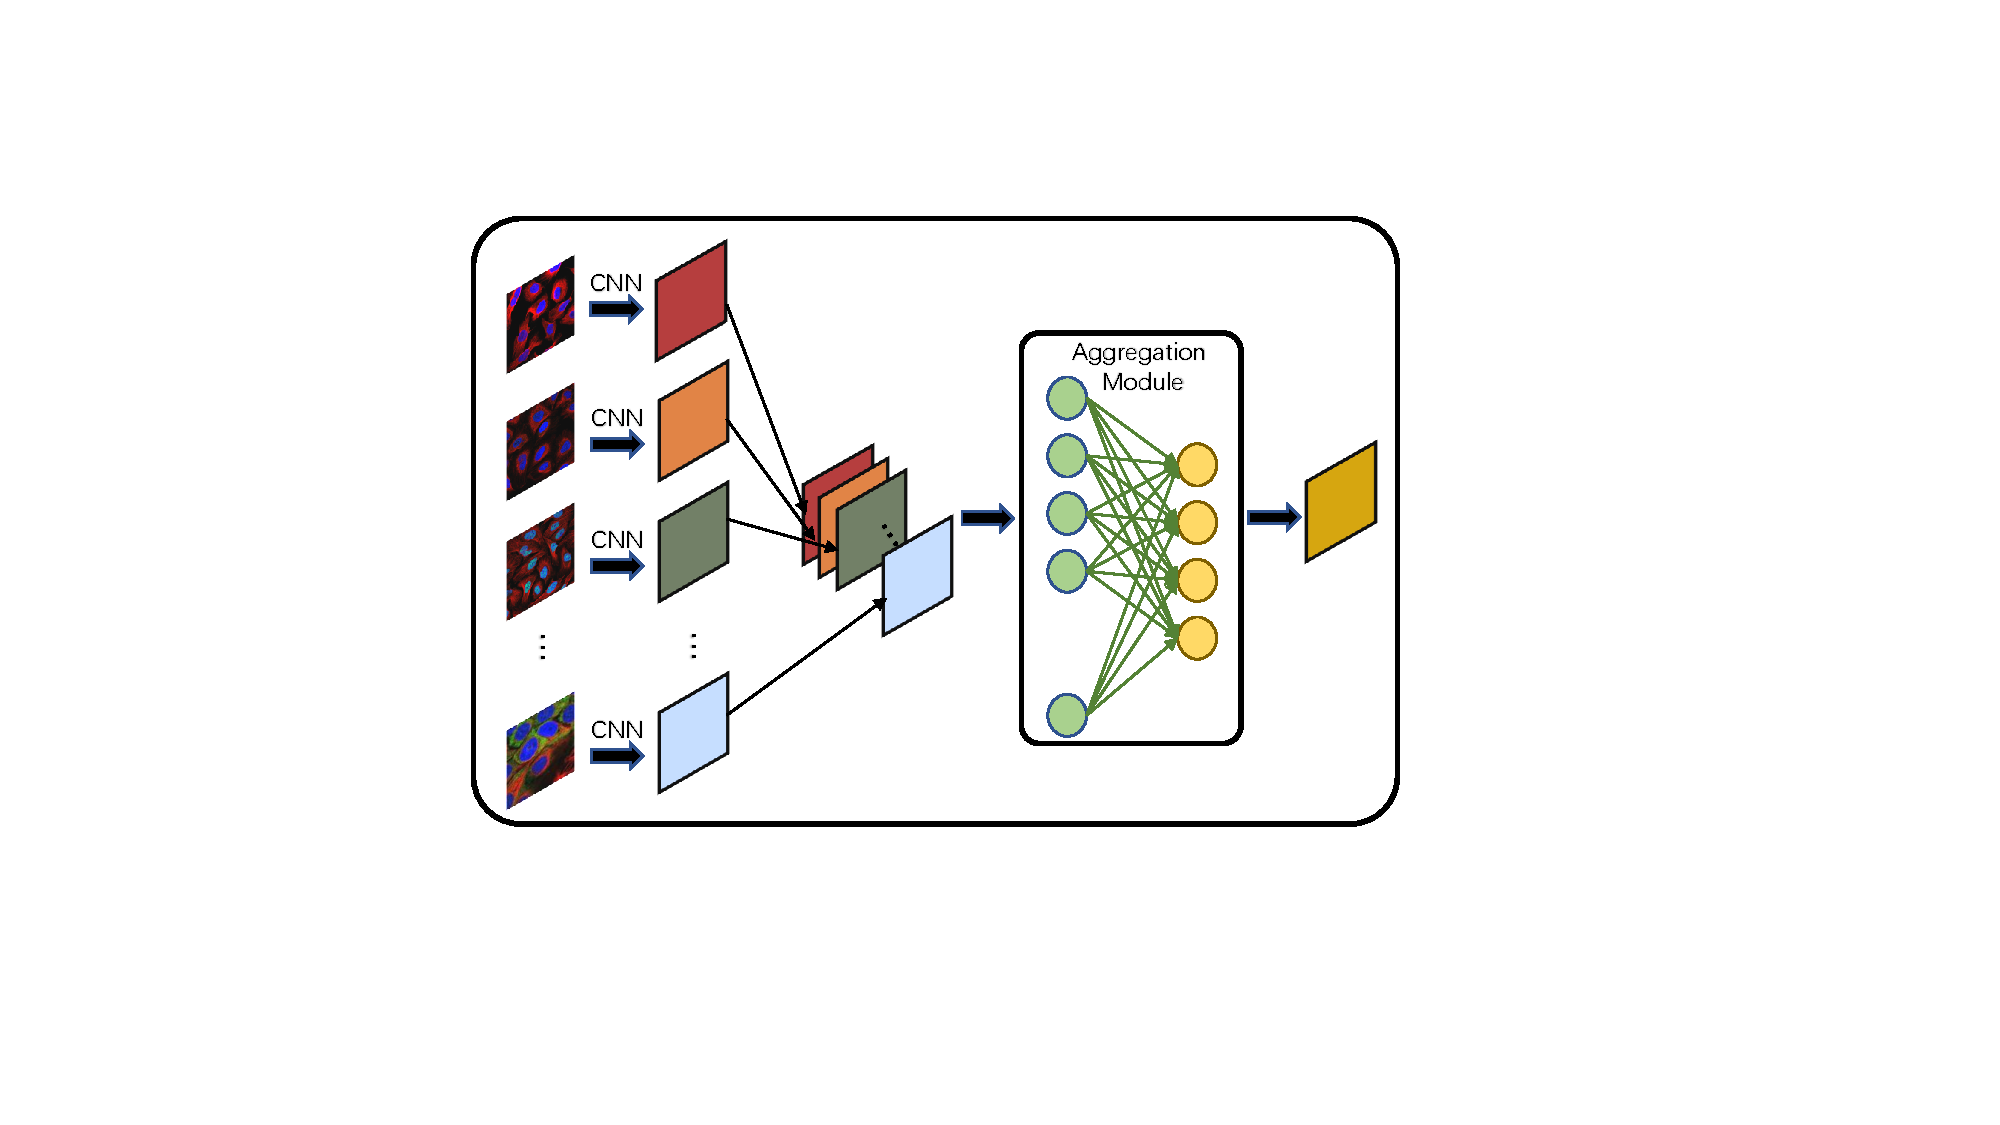
\includegraphics[width=0.8\linewidth]{introduction.pdf}
\end{center}
  \caption{A simple schematic of feature aggregation,The pretrained CNN model is used to extract features from the input images, and then the extracted features are input into the feature aggregation module to obtain the final aggregation output. }
\label{fig:long}
\label{fig:onecol}
\end{figure}

Such multi-image-input (MII) tasks are especially common in the biomedical field \cite{annofly, MIMT-CNN, li2012drosophila, ref27}. 
Benefitting from recent advances of microscopic imaging technology, various types of biomedical images have accumulated at an unprecedented rate for the past decade \cite{ref11,ref12,ref13,ref14}. Image analysis has become a common approach in not only medical diagnosis but also fundamental biological researches from tissue level down to the cell level. Unlike natural images, biomedical images are often much harder to obtain due to the difficulty in preparing the specimen or stringent experimental conditions. Therefore, during the imaging procedure, it is common to capture multiple images for a specimen in a single trial of experiment and perform multiple trails for repeatability. To infer the functions of genes or characteristic of molecules, all the captured images should be considered comprehensively to give a more accurate judgement on the final output, as single images may only contain partial information and it is important to capture the correlation between images, e.g. the 3D structure inference of biomacromolecules using 2D projection images captured from multiple orientations. It is difficult to develop computational methods for addressing MII tasks. The challengs mainly come from variable-sized input and enven image quality.


%For one thing, each data sample is represented by a bag of images where the number of images  is unfixed; and for another, the quality of images varies, i.e. high-quality images and uninformative images are mixed together in the same bag. 
%
%r the MII tasks, there are two major computational challenges.
%\begin{itemize}
%\item i) Variable input bag size. In MII tasks, the number of input images is usually nonfixed, especially when the bags differ greatly in their sizes, which adds difficulty to machine learning models.
%\item ii) Uneven quality of images. Usually, high-quality images and uninformative images are mixed together in the same bag. Thus, how to make the model focus on important images and ignore irrelevant information is a key issue in MII tasks.
%\end{itemize}

The existing approaches to deal with MII learning tasks fall into 3 categories.

i) \textbf{Multi-instance learning (MIL) models.} The MII learning tasks can be regarded as a special kind of problems in machine learning, namely multi-instance learning \cite{zhou2004multi}. As MIL is a general learning framework, it can deal with any type of multi-instance input, such as image \cite{zha2008joint}, text \cite{zhou2005multi}, and chemical structures \cite{dietterich1997solving}. MIL algorithms compute pair-wise similarity or loss function at the bag-level instead of instance-level. Till now, a lot of MIL methods have been developed, like multi-instance KNN \cite{wang2000solving} and multi-instance support vector machines (SVMs) \cite{andrews2003support}. Before using these traditional learning models, image features should be extracted separately. Recently, a deep-learning-based MIL model has been proposed, called DeepMIML \cite{Feng2017AAAI}, but it was designed for single-image input and each image is regarded as a bag of objects. 

  
ii) \textbf{Feature aggregation methods.} Instead of adapting learning models to multi-instance inputs, this type of methods focuses on feature representation. There are a few ways to combine instance-level features to bag-level representation. For instance, in image retrieval, researchers aggregated the patch-based local descriptors into a global descriptor \cite{bov, fishervector, vlad}. Moreover, deep learning models can conveniently achieve feature aggregation by simply using pooling, summation or averaging operations \cite{ref23}. %Some state-of-the-art models are introduced in details in Section \ref{sec:related}.

iii) \textbf{3D data learning models.} Recent advances of deep learning methods allow a more straightforward processing of high-dimensional data. For instance, instead of regarding the input as a bag of images, a 3D convolutional neural network (CNN) model learns 3D data samples directly \cite{kamnitsas2017efficient}.


Apparently, the third type of methods is more suitable for processing video or 3D structural data, in which the images have strong correlations with each other. The first type of methods are mostly traditional shallow learning models. For dealing with image data, extra feature engineering is required. By contrast, the second type is more versatile, including both traditional and deep learning-based models, and can be applied to learn representations for various bags of images.

In this paper, we focus on feature aggregation, because of its flexibility in dealing with various types of image sets, especially originated from biomedical studies, and propose a model, called DRAGN (Deep Recusively AggreGation Network). The model is featured by 
a recursive aggregation protocol and simple but effective aggregation units, which can address the learning of input bags with varying size. We assess the performance of DRAGN on two biomedical image processing applications, namely the prediction of protein subcellular localization and spatial gene expression data annotation. On both tasks, DRAGN achieves significant improvement on prediction accuracy compared with other feature aggregation methods and the state-of-the-art predictors for these two tasks 
% 
%The main contributions  can be summarized as follows:
% 
%i) We design a recursive protocol to aggregate features from multiple images, which can address the learning of input bags with varying size.
% 
%ii) 
%First of all, this paper proposes a general framework for feature aggregation of multi-input single-output design pattern models. This framework has two variants,pre-aggregation and post-aggregation, both of which can effectively conduct feature aggregation.
%
%Secondly, this paper proposes a new feature aggregation module, which includes network complexity optional feature aggregation units and a new feature aggregation process. The feature aggregation module can handle multiple input samples with different length, so that the network is no longer limited by the fixed input samples number.
%
%Finally, we conducted experiments on the human protein atlas data set and the flyexpress data set, and we compared the experimental results with other relevant studies. The experimental results proved that our feature aggregation module has quite obvious advantages in improving the performance of the downstream tasks.

%%%%%%%%%%%%%%%%%%%%%%%%%%%% 2, relate work %%%%%%%%%%%%%%%%%%%%%%%%%%%%%%%%%%%%
\section{Relate Work}
%Feature aggregation is fairly common in the field of computer vision. In video monitoring and face recognition tasks, if multiple photos of the same person taken by different cameras can be sent to the network model for training at the same time, the generalization ability of the model will be greatly enhanced and the accuracy of model recognition will be improved. This will make it easier for the network to grasp the correlation between different images of the same person than send single image to the network for training, while, this correlation information is the key factor for the network to make a right judgement.
Feature aggregation is not a new problem in computer vision. It is used to be a part in feature engineering in traditional methods, and it also benefits from recent advances of deep learning techniques.


\subsection{Traditional methods} 
In traditional image processing, feature aggregation aims to fuse features extracted from single images into a comprehensive feature representation before feeding to a learning model. There are three typical feature fusion methods, namely the bag of visual words (BOV) \cite{bov}, Fisher vector \cite{fishervector}, and vector of locally aggregated descriptors (VLAD) \cite{vlad}. BOV regards image features as words, builds a vocabulary of local image features and generates a vector of their occurrence counts. The Fisher vector method stores the mixing coefficients of the Gaussian mixture model (GMM) as well as the mean and covariance deviation vectors of the individual components. The VLAD method computes the distance of each feature point to the cluster center closest to it. All of these three methods produce a fixed-length feature vector for the input image set, which can work with traditional machine learning models, like SVMs.


%%%%%%%%% 第二个模块大图 %%%%%%%%%%%%%%%%%%%%%%%%%%%
\begin{figure*}
\begin{center}
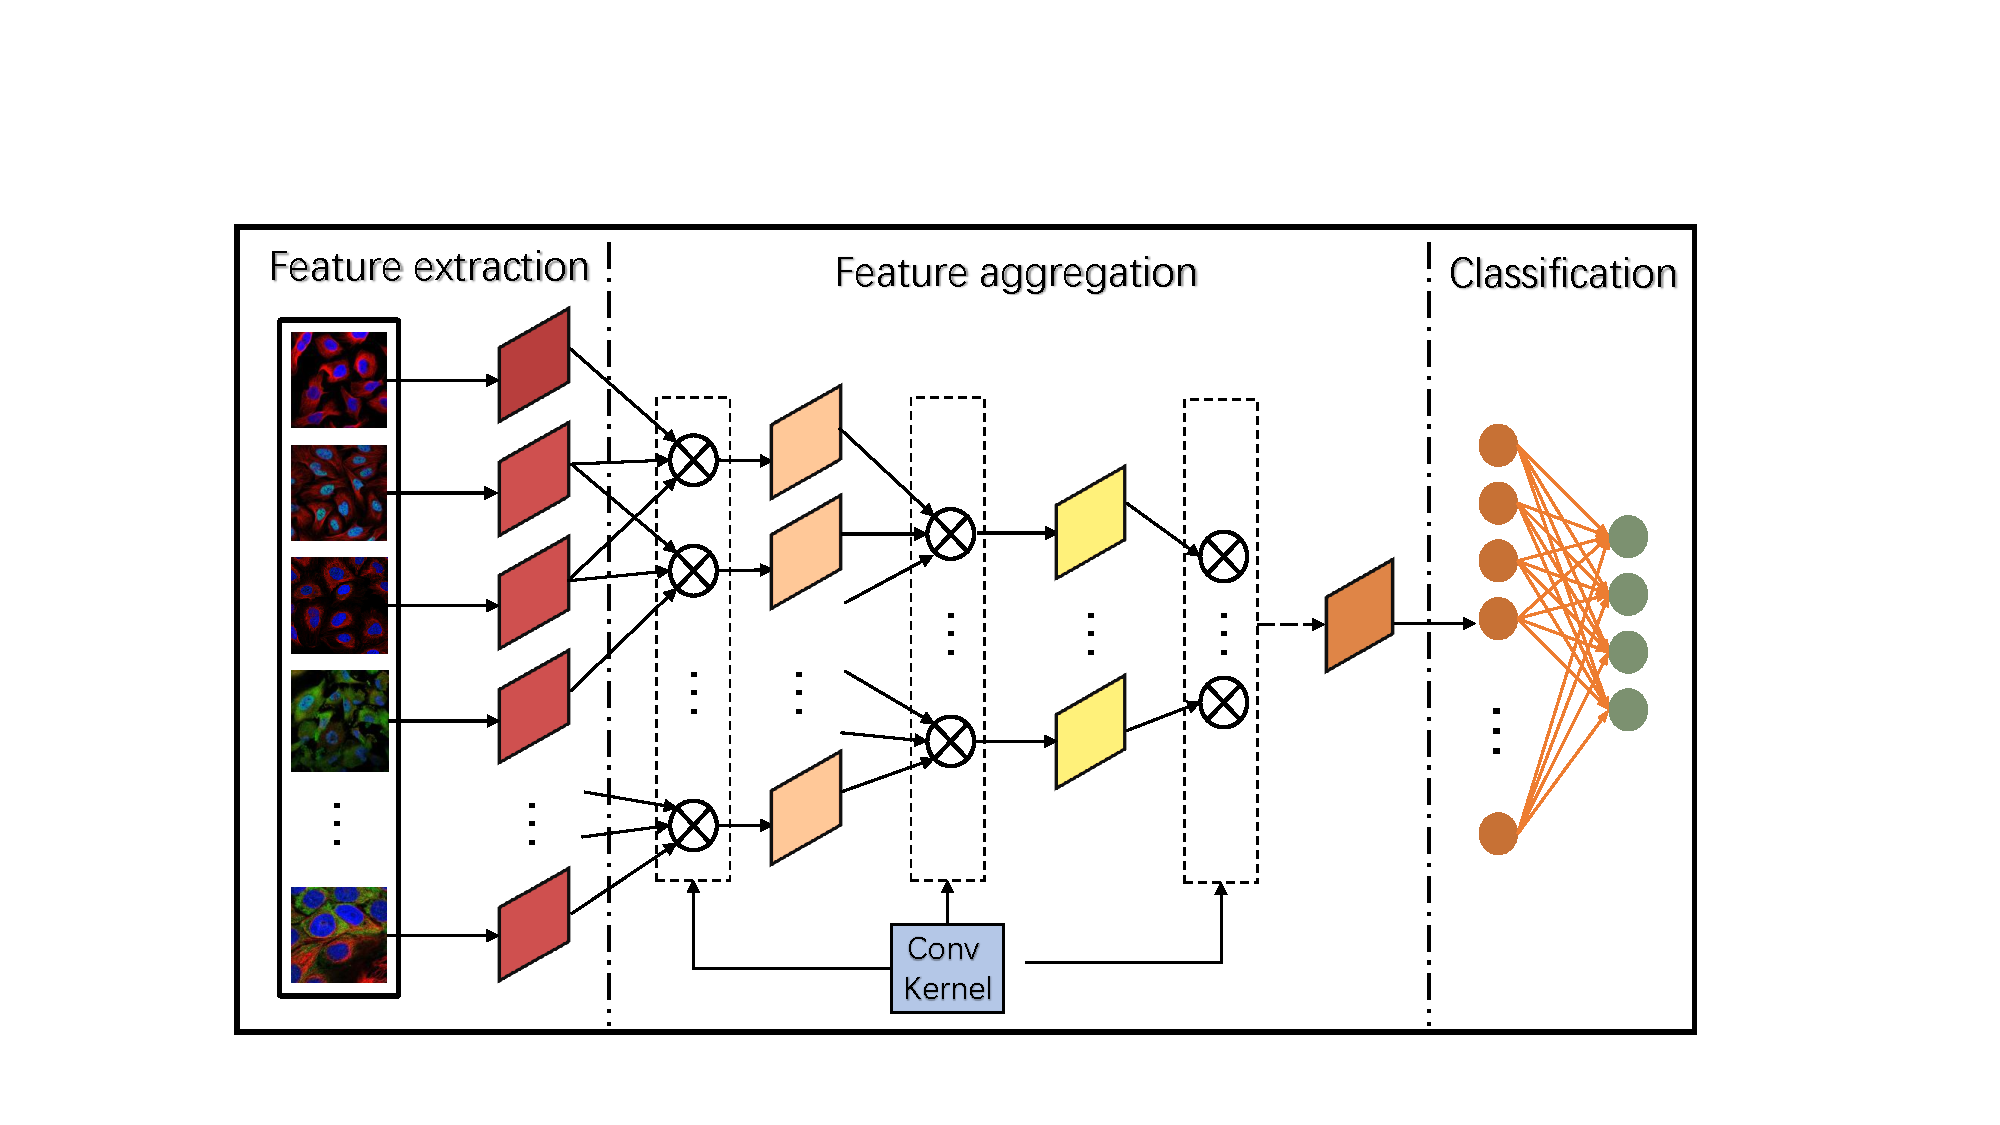
\includegraphics[width=0.8\linewidth]{FlowChart.pdf}
\end{center}
   \caption{Flowchart of post-aggregation methods}
\label{fig:framework}
\end{figure*}

\subsection{Deep learning-based methods}
For the past decade, feature encoding via deep neural networks has almost replaced traditional feature engineering in image processing \cite{ref16, ref19, ref20}. Deep learning-based feature aggregation methods have also emerged, as it is natural to fuse features by using the common operations, like pooling, summation or averaging in convolutional neural networks (CNNs). Su et al. pioneered the studies that integrate feature aggregation into CNNs \cite{ref23}. To achieve 3D recognition by using photos captured from different angles, they designed a Multi-view CNN (MVCNN) model \cite{ref23} to extract photo features and fuse information from multiple orientations. The feature aggregation strategy in MVCNN is simply a maximization operation but very effective in the task. Later, Yang \emph{et al}. proposed a neural aggregation network for video face recognition, NAN\cite{ref24}, which exploited multiple face images to train the network model. Instead of a simple integration procedure, NAN aggregates multiple features by an attention module, which assigns high attention scores to important features.
Besides, by considering the feature vector of each instance as the input at a time step, Yang \emph{et al}. designed a model called Annofly \cite{annofly} based on recurrent neural network, which also implemented an attention mechanism to make the model focus on high-quality images.

In summary, these three methods aim to weight multiple input features by suitable weighting coefficients, so as to obtain final aggregated features, based on either CNN or RNN network architecture. %The proposed DRAGN model also exploit the CNN model, but it integrates multiple input features into one feature through cyclic convolution.


%%%%%%%%%%%%%%%%%%%%%%%%%%%% 3, methods %%%%%%%%%%%%%%%%%%%%%%%%%%%%%%%%%%%%
%-------------------------------------------------------------------------
\section{Methods}
\subsection{Problem Description}


For a multi-input-image (MII) classification task, we aim to learn a model whose input samples are represented by bags of images (i.e., each sample corresponds to a bag of images) and output vectors denote label probabilities. Let $\mathcal{X}$ denote the sample set, i.e. $\mathcal{X}=\{X_i\}$, where $i \in \{1,2,...,n\}$, $n$ is the number of samples, and $X_i$ is a sample; $X_i=\{x_{i,1}, x_{i,2}, \ldots, x_{i,m}\}$, where $m$ is the number of images of the $i$th sample, $x_{i,j}$ ($j \in \{1, 2, ..., m\}$) denotes an image of $X_i$.
Let $\mathcal{Y}=\{Y_i\}$ be the output space, and $Y_i=\{y_1,y_2, \ldots, y_k\}$ corresponds to the label set of $X_i$. The goal is to learn a mapping function $f:\mathcal{X}\mapsto \mathcal{Y}$. 

Generally, there are two frameworks to aggregate multiple instances into a fixed-length input for learning models, namely pre-aggregation and post-aggregation, which differ in the order of performing feature extraction and feature aggregation.

Pre-aggregation first combines multiple instances, by organizing them into a certain data structure, and then extract features for the composite data samples. FlyIt \cite{ref27} is a typical pre-aggregation model, which first stitch images belong to the same bag into large images and then extract features from the large images. Since the combination of multiple raw data samples are very complex in most cases, there is often a strong restriction on the number of combined samples. By contrast,  post-aggregation first extract features for raw instances and then perform the aggregation operation, as shown in Fig. \ref{fig:framework}. For instance, MIMT-CNN \cite{MIMT-CNN} employs 10 VGG models to learn feature representation from 10 images respectively, and concatenate them into a bag representation for the following classification. 
 
DRAGN belongs to the second type, and it integrates feature learning, aggregation and classification in a deep recursive neural network.

\subsection{Model architecture}\label{sec:model}
For MII tasks, a major challenge is how to effectively represent the multi-instance input. Most of the existing methods, no matter pre-aggregation or post-aggregation, set a fixed number of instances to feed the model and perform feature fusion in a single run. 
For example, MIMT-CNN concatenates feature representations from 10 images, Annofly designs an RNN model of 10 time-steps and feeds at most 10 images to the RNN to learn an embedding for the images, and FlyIt stitches 4 raw images into large images. 

An obvious limitation of these methods is the lack of flexibility in the model architecture and the weakness in handling highly variable sizes of input bags. In contrast to the fixed-input and single-run schema, DRAGN implements a new protocol and sets no limit on the number of input instances. It recursively runs feature aggregation, where the running times depends on the number of instances. The model architecture is shown in Fig. \ref{fig:framework}.

By regarding the input bag as a sequence of images, DRAGN slides a fixed-width window over the sequence with step size 1. Within each window, a kernel function (defined in Section \ref{sec:fa}) is called to yield an aggregated feature representation for the images within the window. Then these aggregated feature vectors compose a new sequence. The feature aggregation operation is performed in a recursive way until the sequence contains feature representations less than $L$, then an averaging operation is used to get the final representation. The formal description of the recursive procedure is provided in Algorithm \ref{algo}.


\renewcommand{\algorithmicrequire}{ \textbf{Input:}}      %Use Input in the format of Algorithm
\renewcommand{\algorithmicensure}{ \textbf{Output:}}     %UseOutput in the format of Algorithm

\begin{algorithm}
  \caption{ } \label{algo}
  \label{alg:Framwork}
  \begin{algorithmic}[1]
     \REQUIRE
The set of images for an input bag $X_i$. \\
$X_i=\{x_{i,1}, x_{i,2}, \ldots, x_{i,m}\}$,
\ENSURE
Feature representation $O_i$ for the bag $X_i$.
\STATE Let $w$ be the window size, $L$ be the sequence length ($L = m$), and $f_{agg}$ be the aggregation function.
\STATE $L = L-w+1$.
\FOR{each $k\in [1,L]$} 
\STATE $O_k = f(x_k, \ldots, x_{k+w-1})$.
\ENDFOR
\IF{$L < w$}
\STATE{$O_i$= mean($O_k$), $k\in [1,L]$}, return.
\ENDIF
\STATE Goto  Step 2.
 \end{algorithmic}
\end{algorithm}


% 第三个图: 特征聚合单元
\begin{figure}[t]
\begin{center}
% \fbox{\rule{0pt}{2in} \rule{0.9\linewidth}{0pt}}
  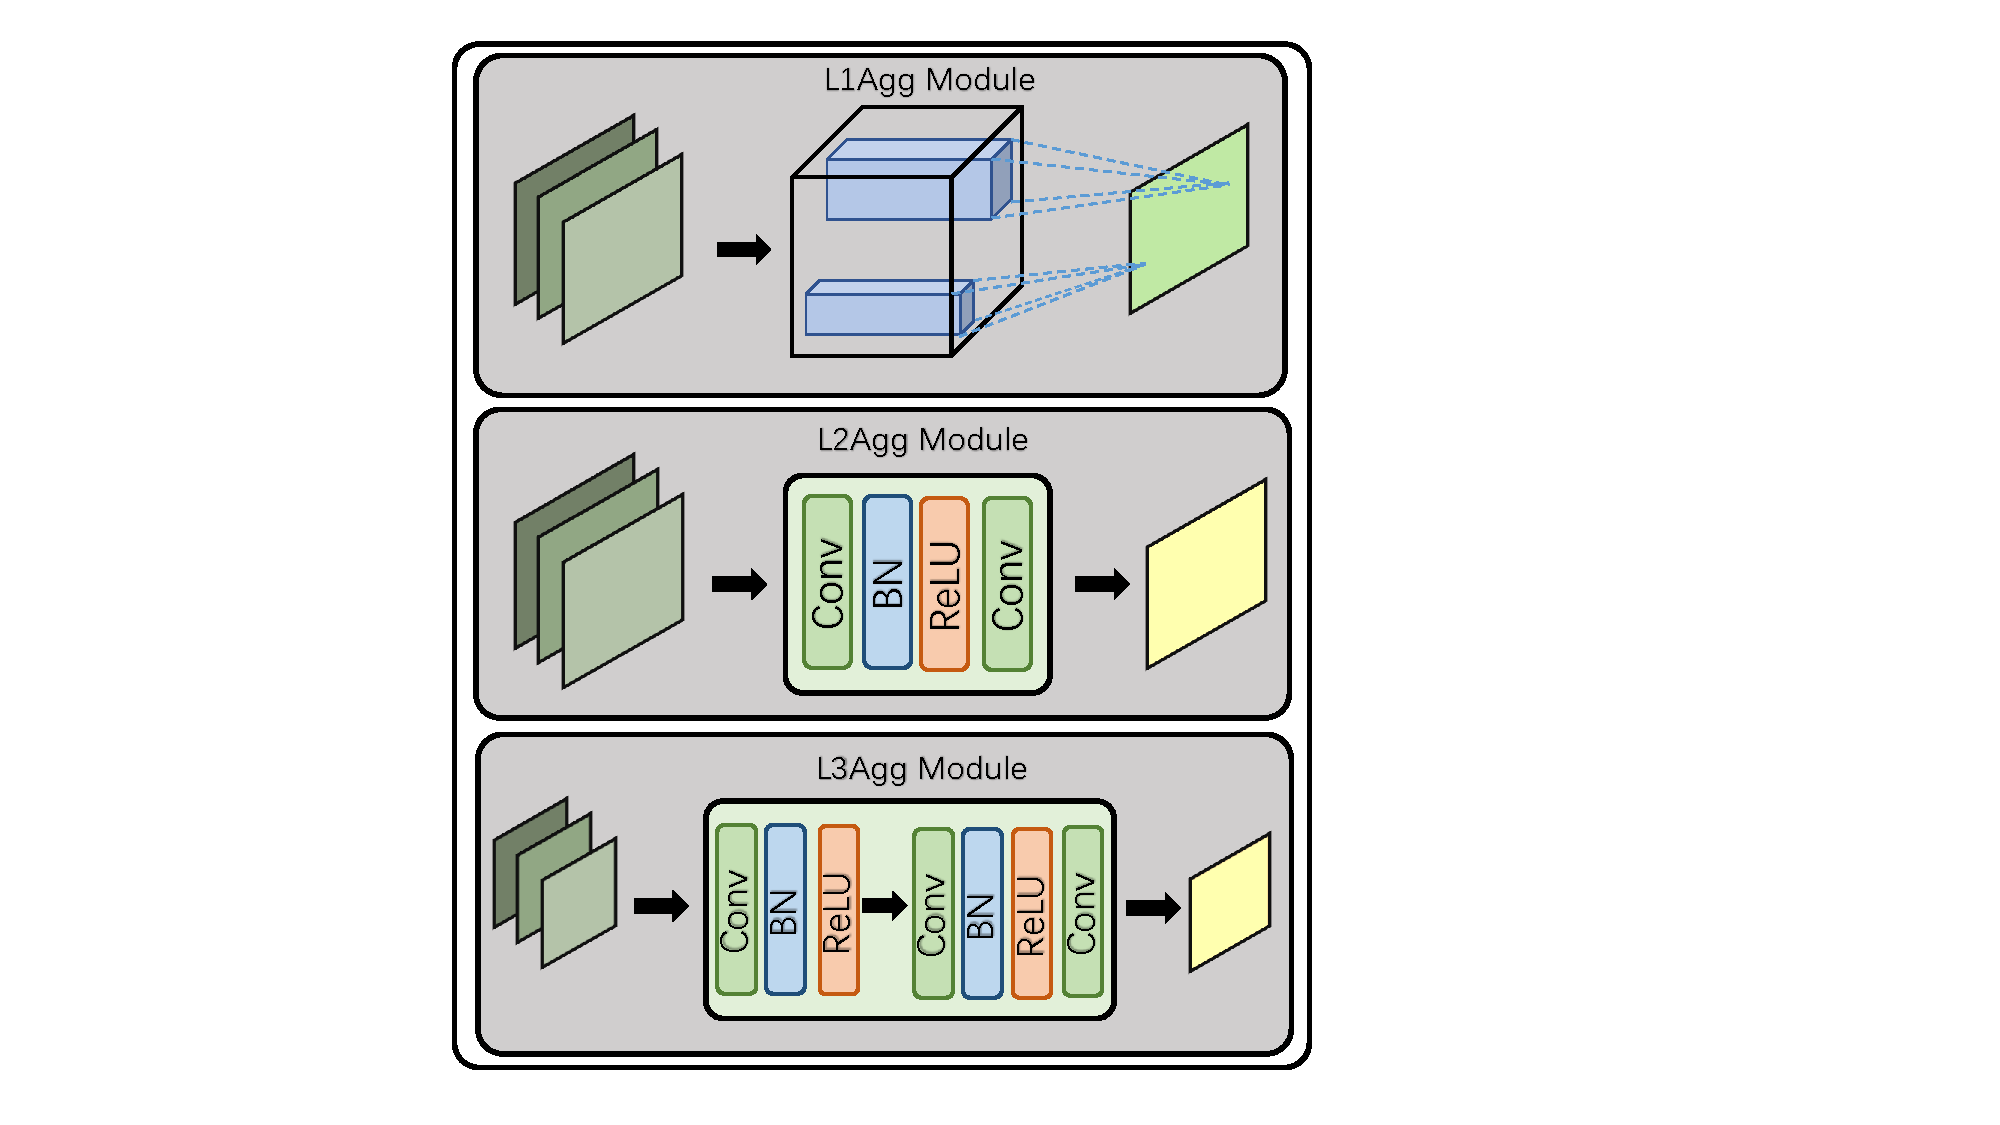
\includegraphics[width=0.8\linewidth]{aggregationUnit.pdf}
\end{center}
   \caption{Feature aggregation unit}
\label{fig:long}
\label{fig:units}
\end{figure}


%%%%%%%%%%% 3.2.1 Feature aggregation unit %%%%%%%%%%%
\subsection{Feature aggregation unit} \label{sec:fa}
The aggregation units in DRAGN mainly involve convolution computations. Formally, let $x_{1}, x_{2}, \ldots, x_{n}$ be the feature maps to be aggregated, where $n$ is the number of feature maps. The aggregation is defined in Eq. (\ref{eq:agg}),
%\begin{equation}
%%\begin{aligned}
%Y'_{i,j} = f'(x_{i,j}),
%Y_i = \bigcup_j Y'_{i,j}, i \in \{1, \ldots, n\}, j \in \{1, \ldots, m\}.
%%1 \leq i \leq n, 1 \leq j \leq m.
%%\end{aligned}
%\label{eq:agg}
%\end{equation}

\begin{equation}
\begin{split}
&\textbf{X}=[x_{1}, x_{2}, \ldots, x_{n}],\\
&O= \textbf{X}*\textbf{W}+b,
%&i\in\{1,2, \cdots, l-h_f+1\}, j \in \{1, 2, \cdots, n\}
\end{split}
\label{eq:agg}
\end{equation}
where $\textbf{X}$ is a tensor composed by the feature maps, $*$ is the convolution operator, $\textbf{W}$ is the convolutional filter, $b$ is the bias, and $O$ is the aggregated feature map. %After the convolution operation, \textbf{y}_i^j turns out to be a column vector, 

We call the feature aggregation unit as L1Agg. To meet the needs from different tasks, in addition to L1Agg, we design two other more complex aggregation units, namely L2Agg and L3Agg, defined in Eqs. \ref{eq:l2} and \ref{eq:l3}, respectively. 

\begin{equation}
O= \textbf{W}*f(g(\textbf{X}*\textbf{W}+b))+b,
\label{eq:l2}
\end{equation}
where $g(\cdot)$ is a normalization function, $f(\cdot)$ denotes the ReLU function.
%
\begin{equation}
O= \textbf{W}*f(g(\textbf{W}*f(g(\textbf{X}*\textbf{W}+b))+b))+b,
\label{eq:l3}
\end{equation}


As shown in Fig. \ref{fig:units}, these three types of units differ in complexity, whereas their working mechanism is the same. And, during the recursive procedure, the convolutional kernel parameters are shared by all aggregation operations.

%According to the requirement of different network complexity, we proposed three feature aggregation units, namely, L1Agg, L2Agg, L3Agg, among which the simplest is L1Agg, whose network model is shown in figure 3. As shown in the figure 3, it contains a convolution layer that receives the input of three features and gives an output feature after convolution. The next is L2Agg and L3Agg. Their network models are shown in figure 4, their netowrk models are respectively consist of conv + BN + relu + conv, and conv + BN + relu + conv + BN + relu + conv. As you can see, they are identical in usage, except for the complexity of the network model.

% % 第四个图: L2Agg 和 L3Agg
% \begin{figure}[t]
% \begin{center}
% % \fbox{\rule{0pt}{2in} \rule{0.9\linewidth}{0pt}}
%   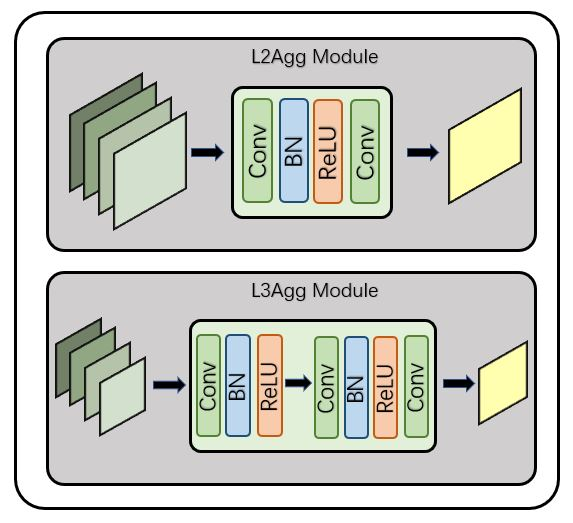
\includegraphics[width=0.8\linewidth]{figure5.JPG}
% \end{center}
%   \caption{Feature aggregation module: L2Agg module and L3Agg module }
% \label{fig:long}
% \label{fig:onecol}
% \end{figure}

% % 第五个图: 特征融合过程算法
% \begin{figure}[t]
% \begin{center}
% % \fbox{\rule{0pt}{2in} \rule{0.9\linewidth}{0pt}}
%   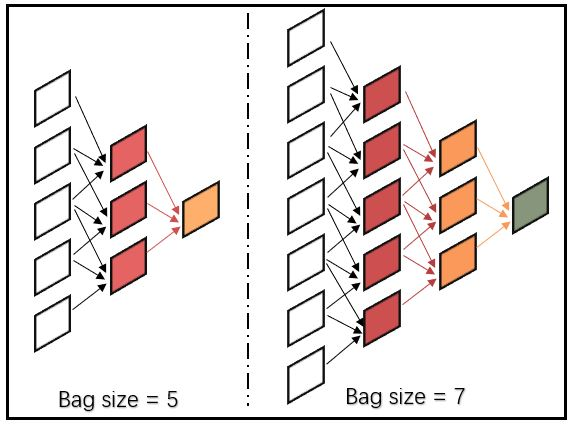
\includegraphics[width=1.0\linewidth]{agg_process.JPG}
% \end{center}
%   \caption{Two examples of Feature aggregation proceses}
% \label{fig:long}
% \label{fig:onecol}
% \end{figure}


%%%%%%%%%%%%%%%%%%%%%%%%%%%% 4, Experiments %%%%%%%%%%%%%%%%%%%%%%%%%%%%%%%%%%%%
\section{Experiments}
We assess the performance of DRAGN on two MII tasks. The first task aims to predict protein subcellular localization based on immunofluorescence (IF) microscopic images. As it is known that, the location information of proteins in the cells is very important for revealing protein functions. Microscopic images can visualize complex localization patterns of proteins, thus make the prediction more accurate and allow tissue-specific studies. This is a typical MII task. Each protein corresponds to multiple microscopic images, and the labels, i.e. cellular locations, are predicted based on all localization patterns implied in these images. However, most of the existing methods convert it into a common image-annotation task. As in the Kaggle competition for classifying subcellular protein patterns in human cells held in January 2019 (www.kaggle.com/c/human-proteinatlas-
image-classification), the contest task is to assign location labels to single images. Here we predict labels at the protein-level via the proposed feature aggregation method, and compare with both single-instance learning models and other feature aggregation models.

The second task aims to assign functional annotation terms to genes based on their expression images, which visualize spatial distribution patterns of gene expression in tissues and help to reveal gene functions. Similar to the first task, the annotation is at the gene-level, and each gene has a set of expression images captured in different angles or experimental trials. We compare the performance of DRAGN on a large-scale gene expression dataset of \emph{Drosophila} embryos with the state-of-the-art methods designed for this annotation task.

%%%%%%%%%%% 4.1, Hpa Experiments %%%%%%%%%%%%%%%%%%%%
\subsection{Task 1: Prediction of protein subcellular localization}

%%%%%% 4.1.1, Dataset introduction %%%%%%
\subsubsection{Data source}
The datasets of Task 1 are collected from the cell atlas of human protein atlas (HPA) database \cite{uhlen2010towards}. We download 1600 bags of IF images, each of which corresponds to a protein. The location annotations of proteins are hand-crafted in the database. The total number of images is 19,777. The sizes of raw images include $800\times 800$, $1728\times 1728$ to $2048\times 2048$. Obviously, the large size of images and small numbers of bags bring great computation difficulties. Considering that there are usually multiple cells within an image, we adopt the selective search algorithm \cite{uijlings2013selective} to pick the cellular patches from raw images, for reducing image size and making the model focus on localization patterns within cells in the meantime. As shown in Fig. \ref{fig:hpa}, the algorithm segments out key regions of cells from the non-informative background.
We resize the selected patches into a fixed size $512\times 512$, and construct a new dataset. Besides, for data augmentation, we also split the patches of the same protein into several bags. Finally, we obtain a total of 24,052 bags and 185,169 patches.

% 第五个图: hpa图片数据展示
\begin{figure}[t]
\begin{center}
% \fbox{\rule{0pt}{2in} \rule{0.9\linewidth}{0pt}}
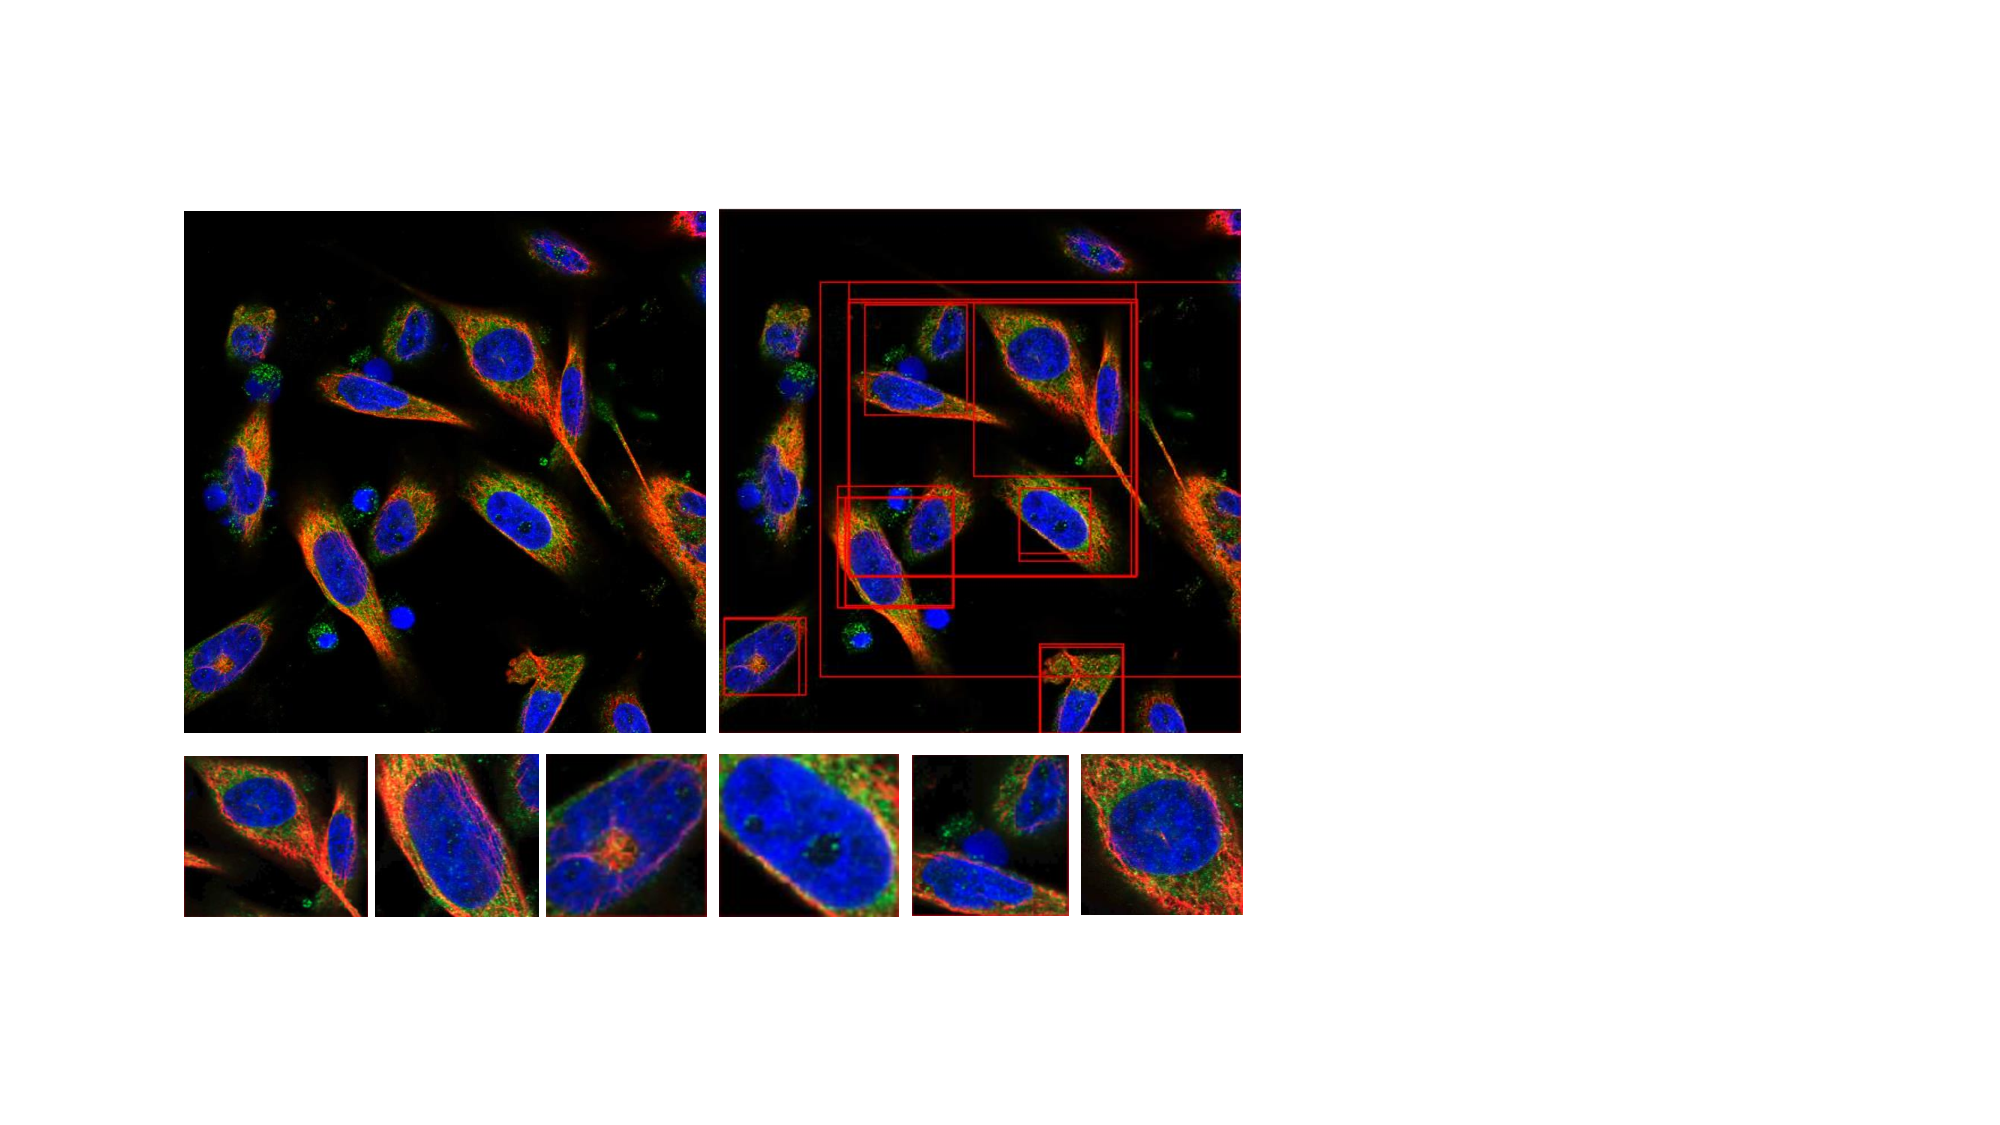
\includegraphics[width=0.9\linewidth]{hpa.pdf}
\end{center}
\caption{Human protein atlas image has size of 2048$\times$2048, and each image contained numerous identical organelles(top left).We use selective search algorithm to pick out the organelle in the original image(top right), and the captured iamges are shown in the bottom. }
\label{fig:hpa}
\end{figure}

%%%%%%%%%%%%%%%%%%%%%%%%%%%%%% 4.13, Experimental Setting %%%%%%%%%%%%%%%%%%%%%%%%
\subsubsection{Experimental Setting}
We implement DRAGN under the pytorch framework on a PC with 2.4GHz CPU, 32GB RAM, and two 2080Ti graphics cards. When optimizing the network, we adopt Adam optimizer \cite{ref25}, we set the learning rate of the network, $\beta_1$, $\beta_2$ to 0.0001, 0.9 and default value respectively. The batch size of the network is set as 16. In this experiment, the loss function is the standard BCE loss. The selected feature extraction network is ResNet50 \cite{he2016deep}, and the final output layer consists of 10 nodes (to predict 10 major cellular organelles). As it is a multi-label classification task (a protein may locate at multiple organelles), we use 5 common multi-label classification metrics, namely AUC value, macro precision, macro recall, macro F$_1$ and micro F$_1$.

%%%%%%%%%%%%%%%%%% 4.1.4, Result and analysis %%%%%%%%%%%%%%%%%%
\subsubsection{Experimental results}
To assess the performance of DRAGN, we compare it with two series models, including two baseline models and 3 other deep learning-based feature aggregation models. 

The two baseline models share basic model component and settings with DRAGN. The first baseline model is a single-instance learning model, denoted by SI, i.e., the input is a single image. As previous works, by transferring the bag labels to all the images in the bag, the model learns a mapping from single images to location labels. In the test phase, for each bag, the images within the bag are predicted one by one, and their results are integrated (maximum values are extracted) to yield the final labels for the bag. The second baseline model adopts the same training mode as DRAGN, except that it simply averages multiple features for feature aggregation, named MI. 

The deep learning-based feature aggregation models, include MVCNN \cite{ref23}, NAN \cite{ref24}, and SPoc \cite{ref28}. MVCNN takes the maximum value of multi-instance features for aggregation, NAN learns adaptive weights between multi-instance features by introducing an attention mechanism, SPoc uses radial basis functions to aggregate multi-instance features. 

The experimental results are shown in Table \ref{tab:base}. As can be seen, the performance of SI is extremely poor on this task, suggesting the advantages of feature aggregation for multiple images over single-instance learning on the MII tasks. MI, MVCNN and DRAGN adopt different aggregation strategy. The first two methods use the average and maximum value in the aggregation, respectively. MI performs the worst, while MVCNN and DRAGN have very close performance. However, MVCNN has a much lower macro F$_1$ than DRAGN. The potential reason is that MVCNN may have an uneven prediction performance for major and minor classes (macro F$_1$ is average F$_1$ over classes). As MVCNN takes maximum values of features, it focuses more on the dominant patterns, whereas the minor classes usually correspond to infrequent patterns, thus has relatively low accuracy. 



%%%%%%%%%%%%% table 1 %%%%%%%%%%%%
\begin{table}
\normalsize
\begin{center}
\begin{tabular}{|l|r|r|r|}
%\hline
%Method & SI & MI & MVCNN & NAN & SPoc & DRAGN \\
%\hline\hline
%AUC(\%) & 95.56 & 95.59 & 96.08 & 95.86 & 93.35 & \textbf{96.56} \\
%\small{macro precision(\%)} & 65.45 & 86.67 & \textbf{91.58} & 81.43 & 79.21 & 90.13 \\
%\small{macro recall(\%)} & 20.96 & 54.23 & 53.59 & 50.85 & 45.86 & \textbf{56.06}\\
%macro F$_1$(\%) & 27.95 & 62.56 &62.75 & 58.18 & 54.72 & \textbf{65.15} \\
%micro F$_1$(\%)& & & \textbf{81.79} & 77.82 & 75.97 & 81.69 \\
%\hline

\hline
Method & AUC(\%) & Macro F$_1$(\%) & Micro F$_1$(\%)\\
\hline\hline
SI & 95.56&  27.95& 68.32\\
 MI & 95.59&62.56& \textbf{81.96}\\
 MVCNN & 96.08&62.7& 81.79\\
NAN & 95.86&58.18&77.82 \\
SPoc &   93.35& 54.72& 75.97\\
DRAGN & \textbf{96.56}& \textbf{65.15}  &81.69\\
\hline
\end{tabular}
\end{center}
\caption{Performance comparison on Task 1}\label{tab:base}
\end{table}



%%%%%%%%%%% 4.2, Drosophila embryo Experiments %%%%%%%%%%%%%%%%%%%%
\subsection{Task 2: Annotation of spatial gene expression patterns}

%%%%%% 4.2.1, Dataset introduction %%%%%%
\subsubsection{Data source}
In this study, we use standard gene expression images of \emph{Drosophila} embryos from the FlyExpress database~\cite{kumar2011flyexpress}. All the images were extracted from the Berkeley \textit{Drosophila} Genome Project (BDGP) (\url{www.fruitfly.org})~\cite{tomancak2002systematic,tomancak2007global} and preprocessed to a uniform size $180\times 320$. We download more than 4000 bags including over 10,000 images. Each bag of images presents the expression distribution on the \emph{Drosophila} embryo for a single gene, in which the images were captured from different orientations, i.e. dorsal, lateral and ventral. We use the dataset as FlyIT \cite{ref27}, where the dataset is divided (at bag-level) into training, validation and test sets according to the ratio of 4:1:5. The total number of labels is 10, each of which is an ontology term describing anatomical and developmental properties. This task is also a multi-label classification problem, as each gene may have multiple developmental terms.


%%%%%% 4.2.3, Experimental Setting %%%%%%
\subsubsection{Experimental Setting}
The experimental settings are almost the same as Task 1, except that we adopt a more lightweight network ResNet18 for feature extraction, due to the smaller size of images and fewer images in bags. 

%%%%%% 4.2.4, Result and analysis %%%%%%
\subsubsection{Experimental results}
As BDGP is the largest gene expression data source, a lot of computational methods have been proposed  for the automatic image annotation in the database. Here we compare DRAGN with the existing approaches, including both shallow learning models and deep neural networks. 



%%%%%%%%%%%%% table 3 %%%%%%%%%%%%
\begin{table}
\footnotesize
\begin{center}
\begin{tabular}{|c|c|c|c|c|c|}
\hline
Method & AUC(\%) & Macro F$_1$(\%) & Micro F$_1$(\%)\\
\hline\hline
ML$_{\text{LS}}$ & 80.92 & 54.99 & 60.17 \\
%PMK$_{\text{SIFT}}$ & 76.73 & 43.31 & 54.60 \\
PMK$_{\text{comp}}$ & 76.66 & 50.02 & 55.86 \\
LR$_{\text{SOFT}}$ & 82.95 & 57.72 & 62.28 \\
%PMK$_{\text{star}}$ & 76.42 & 48.81 & 54.55 \\
%PMK$_{\text{clique}}$ & 76.58 & 45.70 & 54.94 \\
%PML$_{\text{kcca}}$ & 76.51 & 34.36 & 48.83 \\
E-MIMLSVM & 84.60 & 59.80 & 64.00 \\
HMIML & 85.30 & 63.98 & 66.73 \\
AnnoFly&93.67&70.17&71.27\\
FlyIT & 93.59 & 71.81 & 71.08 \\ 
DRAGN & \textbf{94.77} & \textbf{74.74} & \textbf{74.79} \\
\hline
\end{tabular}
\end{center}
\caption{Performance comparison on Task 2}\label{tab:task2}
\end{table}

The experimental results are shown in Table \ref{tab:task2}. The first 4 methods are traditional models while the last 4 models are deep learning models. 
ML$_{LS}$ is a method utilizing the shared subspace multi-label formulation and bag-of-words feature extraction~\cite{ji2009bag}. PMK$_comp$ is the pyramid match kernel (PMK) algorithms, where the subscript ``comp'' denotes the composite kernels \cite{ji2009bag}. LR$_{soft}$ is a feature representation scheme based on sparse coding and incorporating the correlations among terms~\cite{ji2009drosophila}. E-MIMLSVM is an MIML algorithm which adapts the kernel function of support vector machines to the MIML scenario~\cite{Li:2012:DGE:2077941.2077950}. HMIML and FlyIT\cite{ref27} both adopt image stitching to combine raw images but use different CNN architectures for learning, thus belong to pre-aggregation methods. AnnoFly \cite{annofly} first extracts features via ResNet, then employs RNN to deal with the multi-instance input, thus it is a post-aggregation model. 
As can been seen, the deep learning models improve the prediction accuracy significantly compared with shallow models. Among the traditional methods,  E-MIMLSVM, which is the only multi-instance model, performs the best. AnnoFly and FlyIT have very close performance. DRAGN outperforms the second best method FlyIT by around 3\% on F$_1$ values and over 1\% on AUC.  This experiment again demonstrates the advantage of the proposed recursive feature aggregation method over previous multi-instance learning schemas.

\subsection{Visualized analysis}
To further investigate the quality of aggregated features by DRAGN, we perform two kinds of visualization analysis. The results are described in the following subsections.

\subsubsection{Aggregated features are more differentiable}\label{sec:vis1}
In the first analysis, we visualize the features representations learned by deep CNN before and after aggregation, by projecting the features onto a 2D space via tSNE algorithm \cite{tsne}. We use the dataset from Task 2. Fig. \ref{fig:raw} shows the 2D distribution of features learned by ResNet. We perform a feature aggregation based on the same features, and Fig. \ref{fig:agg} shows the 2D distribution of aggregated features. Different colors denote different classes. Note that as Fig. \ref{fig:raw} shows the distribution of single images, while Fig. \ref{fig:agg} shows the distribution of bags, thus the number of points in Fig. \ref{fig:agg} are much fewer than in Fig. \ref{fig:raw}. It can be seen that the features of different categories before aggregation have small margin and large overlap, which brings great difficulties to subsequent classifiers. After aggregation, samples of different categories are much more separated, with small overlap, which is beneficial for subsequent classification.


% 第6个图: 聚合前的分布
%\begin{figure}[t]
%\begin{center}
% \fbox{\rule{0pt}{2in} \rule{0.9\linewidth}{0pt}}
%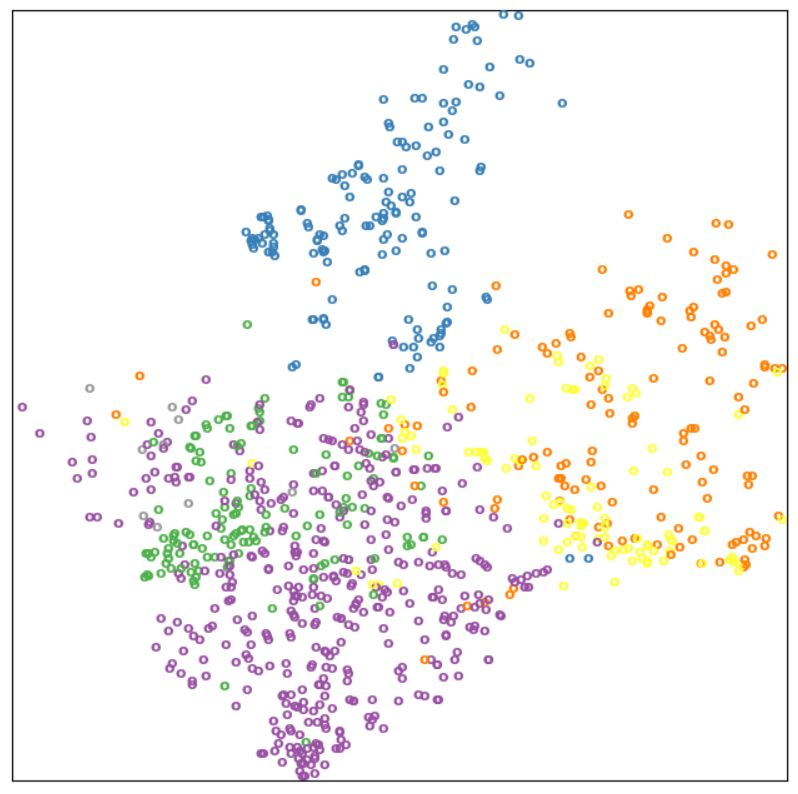
\includegraphics[width=0.9\linewidth]{original.JPG}
%\end{center}
%\caption{the feature distribution before feature aggregation}
%\label{fig:long}
%\label{fig:onecol}
%\end{figure}
%
%
% 第7个图: 聚合后的分布
%\begin{figure}[t]
%\begin{center}
% \fbox{\rule{0pt}{2in} \rule{0.9\linewidth}{0pt}}
%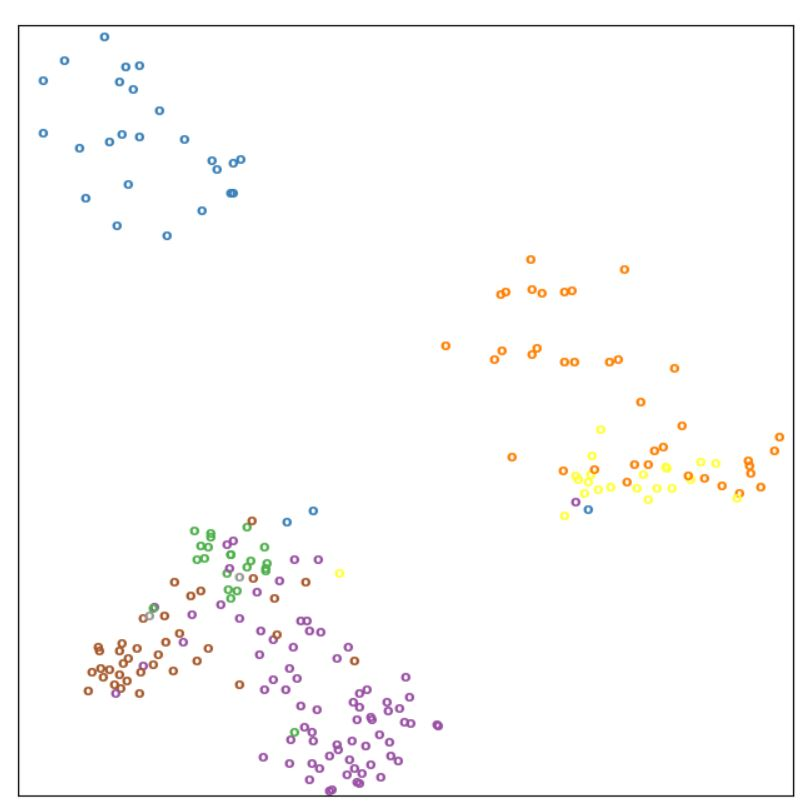
\includegraphics[width=0.9\linewidth]{agg.JPG}
%\end{center}
%\caption{the feature distribution after feature aggregation}
%\label{fig:long}
%\label{fig:onecol}
%\end{figure}
%
%\begin{figure}
%    \centering
%    \begin{subfigure}[b]{0.5\textwidth}
%        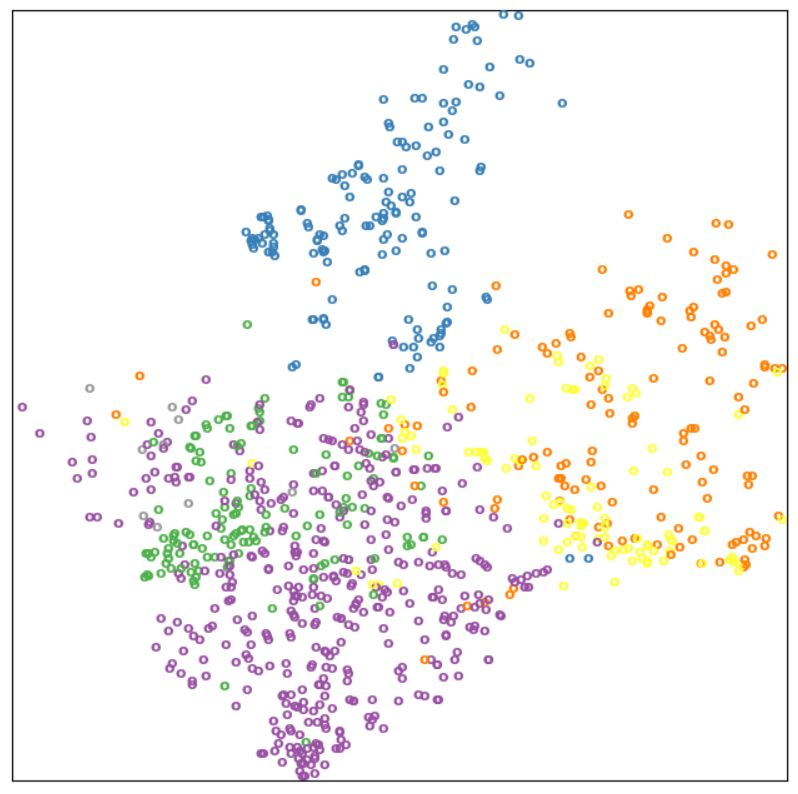
\includegraphics[width=\textwidth]{original.JPG}
%        \caption{Raw image features}
%        \label{fig:raw}
%    \end{subfigure}
%    ~ %add desired spacing between images, e. g. ~, \quad, \qquad, \hfill etc.
%      %(or a blank line to force the subfigure onto a new line)
%    \begin{subfigure}[b]{0.5\textwidth}
%        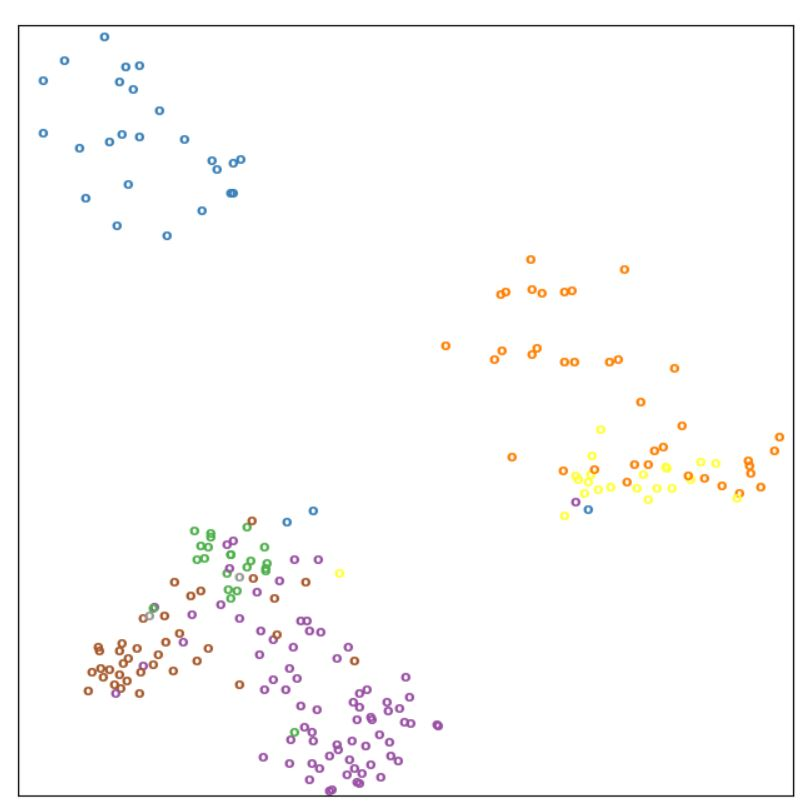
\includegraphics[width=\textwidth]{agg.JPG}
%        \caption{Aggregated features}
%        \label{fig:agg}
%    \end{subfigure}
%      \caption{The distribution of feature representations before and after aggregation}\label{fig:tsne}
%\end{figure}

\begin{figure}
\begin{minipage}[t]{0.25\textwidth}
\centering
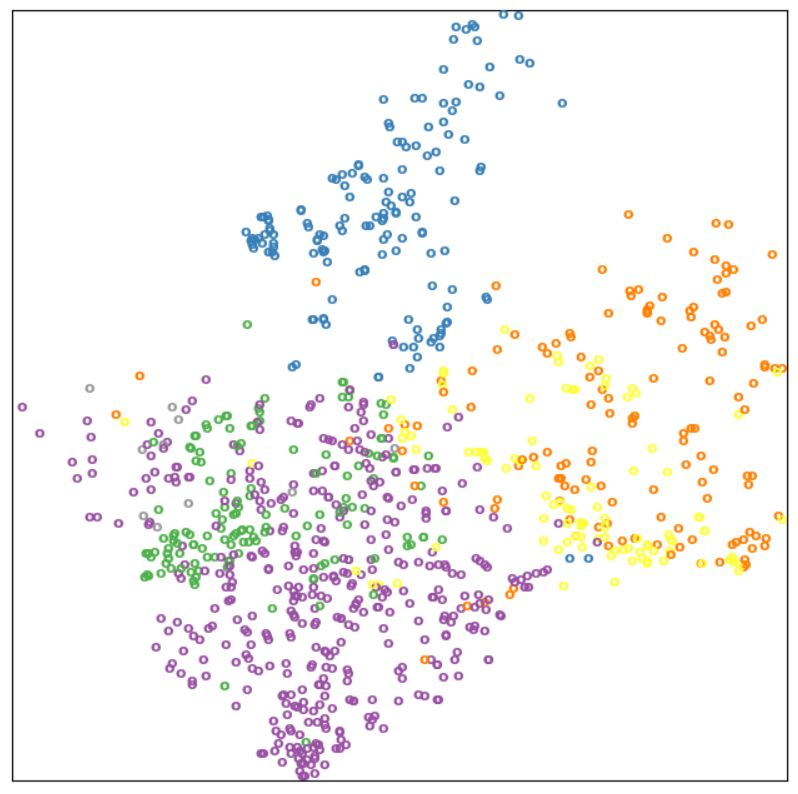
\includegraphics[width=\textwidth]{original.JPG}
\caption{Raw image features}
\label{fig:raw}
\end{minipage}%
\begin{minipage}[t]{0.25\textwidth}
\centering
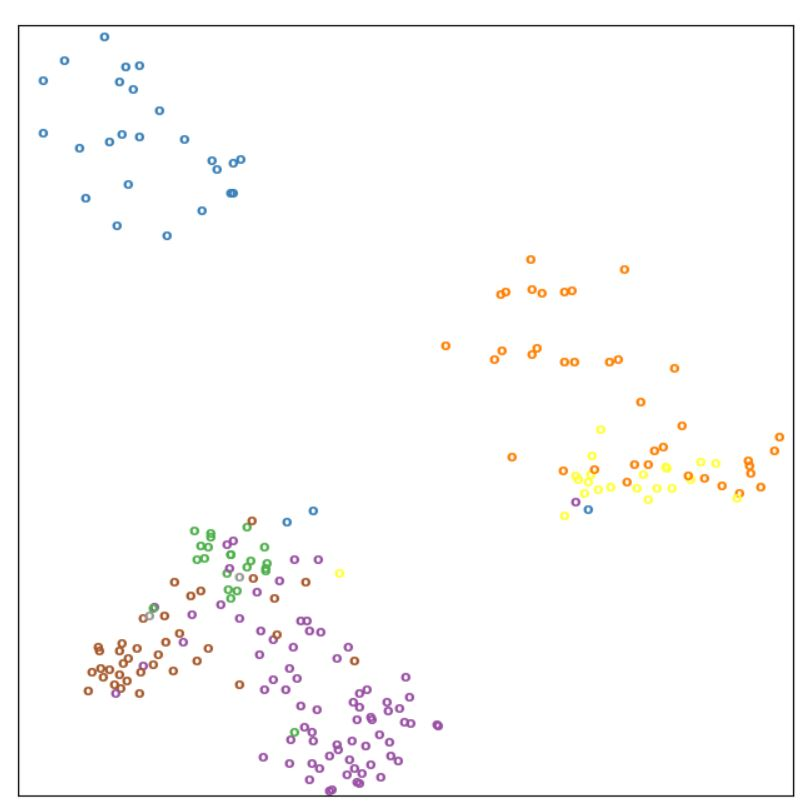
\includegraphics[width=\textwidth]{agg.JPG}
\caption{Aggregated features}
\label{fig:agg}
\end{minipage}
\end{figure}


\subsubsection{Aggregated features retain more information from high-quality images}
From Section \ref{sec:vis1}, we can observe that the feature aggregation make the image patterns more distinguishable. In order to
get more insight on the aggregation operation, we compute the cosine similarity between aggregated features and the features of input images, and take the similarity value as the score of the input images. Fig. \ref{fig:vis2} visualizes the images with different scores. Each row shows images from the same bag, the first column lists typical labels for the bag. As can be seen, the images with high scores contain relatively obvious local patterns corresponding to
the target labels, suggesting the feature aggregation retain more information from the high-quality images, i.e.  the features aggregated by DRGAN will automatically focus on important features.


% 第8个图: 可视化权重
\begin{figure}
\begin{center}
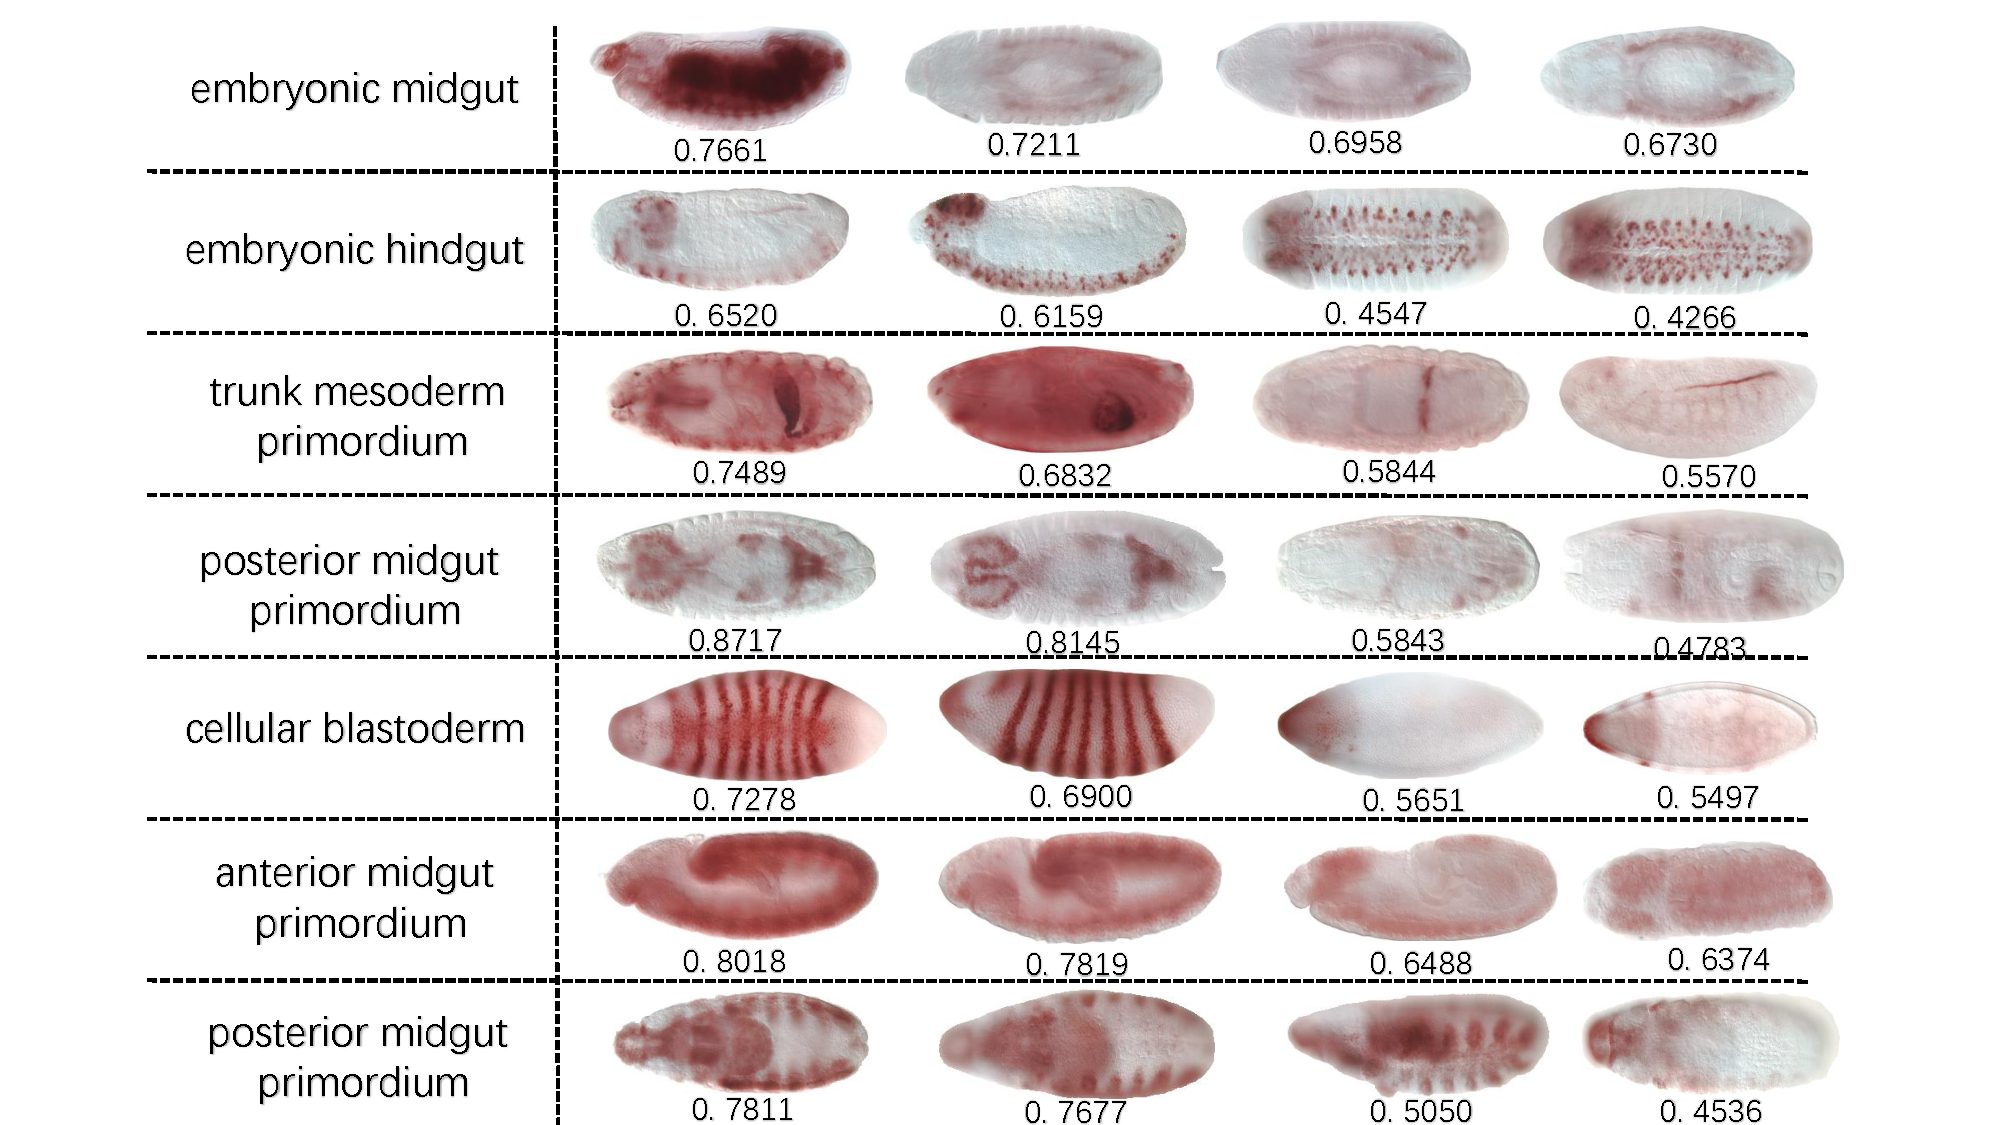
\includegraphics[width=0.8\linewidth]{flycompare.pdf}
\end{center}
   \caption{The weight distribution between the aggregated feature and the original images.}
\label{fig:vis2}
\end{figure}


%-------------------------------------------------------------------------

%%%%%%%%%%%%%%%%%%%%%%%%%%%% 5, Conclusion and Discussion %%%%%%%%%%%%%%%%%%%%%%%%%%%%%%%%%%%%
\section{Discussion and conclusion}
This paper proposes a general network framework DRAGN for dealing with the MII problems. DRAGN is featured by a deep recursive architecture and convolution-based aggregation unit. The advantages of DRAGN are summarized as follows.

i) High accuracy and good applicability to various multi-instance image classification tasks;
ii) The flexibility of allowing variable sizes of input bags without a restriction on the bag size.
iii) Simplicity in aggregating features.

Although our model has shown excellent performance in both of these two tasks, but the scope of our model is not limited to these two tasks. The DRAGN we proposed is a general feature aggregation network, we can easily change its components to make it suitable for other tasks and improve their performance. As a future work, we will investigate the impact of recursion depth on the aggregated features, and explore the potential of fusing features generated in different recursion depth to obtain more comprehensive feature representations.


%%%%%%%%%%%%%%%%%%%%%%%%%%%% 6, Future Work %%%%%%%%%%%%%%%%%%%%%%%%%%%%%%%%%%%%
%\section{Future Work}
%Although the experiments in this paper are carried out based on images from the biological field, our model is a general framework and not only confined to the biological field. As we described in the introduction, there are also scenes using feature aggregation in the field of natural images.Therefore, in the feature, we will consider applying DRAGN proposed in this paper to the field of natural images in order to improve the performance of related tasks.
%
%In the future, we will also explore to use the our model to the field of biological sequences. Since most biological sequences domains have temporal information, we will consider to use RNN to design the feature aggregation units to capture temporal information between multiple features in the biological sequence domain. In this way, multiple biological sequences features can be effectively integrated to improve the metrics and performance of related tasks in the field of biological sequence.

%%%%%%%%%%%%%%%%%%%%%%%%%%%% 7, reference %%%%%%%%%%%%%%%%%%%%%%%%%%%%%%%%%%%%
{\small
%\bibliographystyle{ieee_fullname}
\bibliographystyle{unsrt}
\bibliography{egbib}
}

\end{document}
